% TODO:La fiabilidad en el software
\section{La fiabilidad en el software}
El objetivo final de la \ac{FT}, es el desarrollo de un sistema fiable \citep{FTDesign}. Teniendo 
en cuenta que \ac{SW} que se encuentran dentro de las naves espaciales, como satélites, 
lanzadores, y sobre todo vehículos tripulados son críticos, ya que de ellos dependen el éxito o 
fracaso de una misión, se debe llevar a cabo un sistema fiable. La fiabilidad de un sistema es la 
capacidad del mismo de entregar a los usuarios un nivel deseado de servicio \citep{FTDesign}. 

La fiabilidad también se la puede considerar como una propiedad global que permite justificar la 
confianza de los servicios de un sistema \citep{FTAvionics}. Por lo tanto, como lo indica 
\cite{FTAvionics} la fiabilidad es un término amplio y cualitativo que está relacionado con 
atributos no funcionales (o ``-ilities''), que buscan generar un sistema ``ideal'', especialmente 
cuando su funcionamiento es crítico. 

Como se muestra en la Figura \ref{fig:dependability_relations} la consecuencia de la fiabilidad es 
la relación entre la evitación de fallos y la reducción de fallos, así como también la \ac{FT}.

\begin{figure}[h]
 \centering
 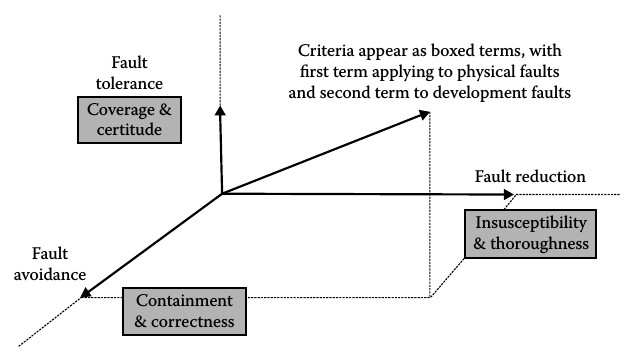
\includegraphics[scale=0.5]{images/Marco_teorico/dependability_relations}
  \caption{Fiabilidad \protect\citep{FTAvionics}}  
\label{fig:dependability_relations} 
\end{figure}

Según \cite{Pullum01} la fiabilidad puede ser clasificada en:
\begin{itemize}
 \item Impedimentos: son aquellas cosas que se interponen en el camino de la fiabilidad. Son las 
fallas, errores y fracasos. 
 \item Medios: los medios para lograr la fiabilidad, según el autor, se pueden dividir en dos 
grupos:
  \begin{enumerate}
    \item Aquellos que son utilizados durante la construcción del \ac{SW} (\ac{FA}\footnote{En 
    inglés, Fault Avoidance} y \ac{FT}).
    \item Aquellos que contribuyen con la validación del \ac{SW} una vez desarrollado 
    (\ac{FR}\footnote{En inglés, Fault Removal} y \ac{FF}\footnote{En inglés, Fault Forecasting}).
  \end{enumerate}

 \item Atributos: describen las propiedades de la fiabilidad y proporcionan una forma de evaluar el 
logro de esas propiedades. 
\end{itemize}

% TODO: deteriodo de la confiabilidad
\section{Impedimentos de la confiabilidad}
El impedimiento de la confiabilidad o deteriodo de la confiabilidad es definido en términos de 
fallas, errores, y fracaso \citep{FTDesign}. Los mismos fueron desarrollados en la sección 
\ref{sec:terminologia}. Lo que tienen en común estos tres conceptos, es que avisan, o dan alerta 
cuando algo está mal \citep{FTDesign}. La diferencia radica, en que las fallas son a nivel físico; 
los errores se dan a nivel computacional; mientras que los fracaso se dan a nivel de sistema 
\cite{FTDesign}.

\subsection{Orígenes de la falla}
Existen diversos orígenes de fallas. Estas pueden provenir desde terceros, en el caso de productos 
comprados, pueden deverse a una falta del conocimiento del problema, falta de tiempo, etc. 
\cite{FTDesign} clasifica el orígen de las fallas en cuatro grupos: \textit{especificación 
incorrecta, implementación incorrecta, defectos de fabricación y factores externos}

Las \textit{especificaciones incorrectas} son aquellas que surgen debidas a una incorrecta 
especificación de requerimiento o un mal diseño de una arquitectura o de un algoritmo 
\citep{FTDesign}. Estos orígenes de fallas son bastante comúnes en el desarrollo de sistemas. Un
ejemplo típico citado por \cite{FTDesign}, es el caso de requerimientos que ignoran aspectos del 
medio ambiente en el que opera el sistema. Una mala redacción de un requerimiento o el olvido de 
uno de ellos, puede traer graves problemas, atrasos y pérdida de dinero,  en el diseño y producción 
de un sistema espacial. 

Las \textit{implementaciones incorrectas}, se refieren a las \textit{fallas de diseño}, surgen 
cuando el sistema implementado no cumple con los requerimientos \citep{FTDesign}.

Otro orígen de falla son los \textit{defectos de los componentes} \citep{FTDesign}.Estos pueden 
incluir defectos de fabricación, defectos aleatorios dados en los componentes, etc.

Y por último se tienen las fallas que son causadas por \textit{factores externos}, los cuales 
provienen del medio ambiente, usuarios u operadores \citep{FTDesign}. Ejemplos de estos factores 
externos pueden ser, vibraciones, cargas electroestáticas, temperatura, radición electromagnética, 
envío incorrecto de comandos, etc.

% TODO: Modos comúnes de fallas
\subsection{Modos comúnes de fallas}
Un \textit{\ac{CMF}}\footnote{En inglés, common-mode faults} es una falla que ocurre 
simultaneamente en dos o más componentes redundantes \citep{FTDesign}. 

\cite{Gangloff75} define los \ac{CMF} como múltiples unidades de fracaso debido a una sola causa. 

\ac{CMF} son causados por fenómenos que crean dependencias entre unidades redundadas, lo que causa 
la falla de estas unidades simultaneamente \citep{FTDesign}. 

Según como lo indica \cite{FTDesign} el único enfoque para combatir los \ac{CMF}, es mediante el 
diseño en diversidad. Diseño en diversidad es la implementación de más de una variante de la 
función en cuestión \citep{FTDesign}. Esto se puede lograr variando los algoritmos que se utilizan, 
diferentes equipos de trabajo realicen las mismas partes del sistema, de manera tal de tener 
redundancia en código, etc. 

%TODO: Fallas en el Software
\subsection{Fallas en el Software}
El \ac{SW} difiere en gran medida con el \ac{HW}. En primer lugar el \ac{SW} no envejece, no se deforma, tampoco se puede quebrar ni ser afectado
por el medio ambiente. El \ac{SW} es determinístico, siempre responde de la misma manera en el mismo ambiente, al menos que falle.

Por otro lado el \ac{SW} se lo puede actualizar varias veces a lo largo del su ciclo de vida. 

En tercer lugar, arreglar bugs de \ac{SW} \textbf{no significa que el mismo sea más confiable}, al contrario pueden ocurrir nuevos errores \citep{FTDesign}.

Por último el \ac{SW} es mucho más complejo y menos regular que el \ac{HW}. Tests tradicionales y métodos de debug pueden ser inadecuados para los sistemas de \ac{SW}

% TODO: medios de fiabilidad
\section{Medios de fiabilidad}
Los medios de confiabilidad son métodos y técnicas que permiten el desarrollo de un sistema 
confiable \citep{FTDesign}. Los medios se pueden dividir en dos grandes grupos \citep{Pullum01}:
\begin{enumerate}
 \item Aquellos que son empleados durante el proceso de construcción del \ac{SW} \citep{Pullum01},
 \item y a quellos que ayudan en la validación del \ac{SW} después que fue desarrollado 
\citep{Pullum01}.
\end{enumerate}

Dentro del primer grupo se tiene:
\begin{itemize}
 \item \acl{FA}
 \item \acl{FT}
\end{itemize}

Por otro lado, en el segundo grupo se puede mencionar los siguientes:
\begin{itemize}
 \item \acl{FR}
 \item \acl{FF}
\end{itemize}

\subsection{\acl{FA}}
\ac{FA} son técnicas de mejoramiento de la fiabilidad utilizadas durante el desarrollo de \ac{SW} 
para reducir el número de fallas introducidas durante la etapa mencionada \citep{Pullum01}. Estas 
técnicas pueden estar presentes en las especificaciones y requerimientos del sistema, métodos de 
diseño de \ac{SW} \citep{Pullum01}.

\cite{FTDesign} la denomina \textit{prevensión de fallas}\footnote{En inglés, Fault prevention}, y 
coincide con el autor anterior, definiendo \ac{FA} como técnicas de control de calidad durante la 
especificación y fabricación de los procesos de diseño. 

% In page 22 of Pullum01 there're more definitions that may be important inside Failure avoidance

\subsection{\acl{FT}}
En la sección~\ref{chap:FaultTolerance} (página~\pageref{chap:FaultTolerance}) se discutirá con 
mayor detalle la \ac{FT}. Esto es así ya que en este trabajo de tesis se tiene como principal punto 
de estudio la \acl{FT}.

\subsection{\acl{FR}}
La \ac{FR} hace referencia a las técnicas utilizadas para mejorar la fiabilidad empleadas durante 
la validación y verificación del \ac{SW} \citep{Pullum01}. Estas técnicas mejoran la fiabilidad del 
\ac{SW} mediante la detección de fallas, usando métodos de verificación y la validación, y 
eliminando las fallas que se van detectando \citep{Pullum01}. 

Por otro lado \cite{FTDesign} indica que el \ac{FR} se lleva a cabo durante fases de desarollo de 
\ac{SW} tanto como durante el ciclo de vida de un sistema. Durante la fase de desarrollo, \ac{FR} 
consiste en tres pasos: \textit{verificación, diagnóstico y correción} \citep{FTDesign}. \ac{FR} 
durante la vida operacional de un sistema, consiste en el mantenimiento preventivo y correctivo del 
mismo \citep{FTDesign}.

\subsection{\acl{FF}}
La \ac{FF} se realiza mediante la realización de una evaluación del comportamiento del sitema con 
respecto a la ocurrencia o la activación de una falla \citep{FTDesign}.Esta evaluación puede ser:
\begin{itemize}
 \item Cualitativa: que tiene como objetivo clasificar los modos de fallas o combinaciones de 
eventos que llevan al sistema al fracaso \citep{FTDesign}. 
 \item Cuantitativa: que tiene como objetivo evaluar en término de probabilidad, el grado en el 
cual los atributos de fiabilidad son satisfechos \citep{FTDesign}. 
\end{itemize}

\ac{FF} incluye técnicas para aumentar la fiabilidad del sistema que son usados durante la 
validación del \ac{SW}, con el objetivo de estimar la presencia de fallas y la ocurrencia o 
consecuencia de fracasos \citep{Pullum01}

% TODO: atributos de la fiabilidad
\section{Atributos de la fiabilidad}\label{sec:atributos_de_la_fiabilidad}
El objetivo final de la \ac{FT} es desarrollar un sistema que sea fiable. Fiabilidad tiene muchas 
definciones, pero comúnmente es expresado como la probabilidad de \textbf{no fallar} 
\citep{FTAvionics}. ``La fiabilidad es la probabilidad de que un sistema continúe funcionando 
correctamente durante un intervalo de tiempo particular'' \citep{SoftwareFaultToleranceATutorial}.

La fiabilidad de un sistema \ac{SW} puede ser descrita por una serie de atributos, los cuales son 
mencionados a continuación.

\subsection{Confiabilidad}\label{subsec:confiabilidad}
La confiabilidad es la probabilidad de que un sistema continua operando correctamente durante un 
intervalo de tiempo dado \citep{SoftwareFaultToleranceATutorial}. 

\cite{FTDesign} coincide que la confiabilidad \textit{R(t)}\footnote{En inlgés, Reliability} de un 
sistema es la probabilidad de que el sistema opere sin fracasos en el intervalo de tiempo 
\textit{[0,t]}. 

La confiabilidad es una medida de la entrega correcta del servicio que brinda un sistema 
\citep{FTDesign}.

En sistemas críticos como el \ac{SW} de vehículo espacial, es sumamente necesario que tenga una 
alta tasa de confiabilidad, ya que por ejemplo, perder el contacto con la nave, podría representar 
la pérdida de la misión, o una gran cantidad de datos. Otro ejemplo que se puede mencionar es de un 
satélite geoestacionario de comunicación, la pérdida de este servicio debe ser baja, casi nula 
(idealmente). 

Coincidiendo \cite{pressman01}, define la confiabilidad como la ``probabilidad de tener operaciones 
libre de fallas de un programa de computadora, en un ambiente específico para un tiempo 
específico''. El mismo autor también indica que la confiabilidad es la \ac{MTBF}\footnote{Del 
inglés, mean-time-between-failure}. Donde:

$$MTBF = MTTF + MTTR$$

\ac{MTTF} es el promedio de tiempo desde que empieza la operación del sistema hasta el tiempo que 
se produce la primera falla. \ac{MTTR} es el promedio de tiempo que se requiere para recuperarse, 
después de un fracaso, al correcto funcionamiento \citep{Hanmer07}. \ac{MTBF}  es similar a 
\ac{MTTF}, lo único que los diferencia es que \ac{MTBF} es la suma de \ac{MTTF} y \ac{MTTR}. Según 
\cite{Hanmer07} \ac{MTBF} es utilizado para aquellos sistemas que son reperables. Para el caso 
contrario se utiliza \ac{MTTF}. 

La \cite{IEEE610.12} define confiabilidad como ``La capacidad del sistema o componente de realizar 
sus funciones requeridas bajo las condiciones establecidas durante un período de tiempo 
especificado''. 

\subsection{Disponibilidad}
Es la probabilidad de que el sistema esté operando correctamente en un determinado instante de 
tiempo \citep{SoftwareFaultToleranceATutorial}. La disponibilidad \textit{A(t)} de un sistema en el 
instante de tiempo \textit{t} es la probabilidad que el sistema esté funcionando correctamente en 
el instante \textit{t} \citep{FTDesign}. 

\cite{FTDesign} realiza un definción matemática de \textit{A(t)}, llamandola también como, 
\textit{punto de disponibilidad} o \textit{disponibilidad instantanea}. Y la define como:

$$A(T) = \frac{1}{T} \int_0^T \! A(t) \, \mathrm{d}x $$

Para \cite{Hanmer07} la disponibilidad del sistema es el porcentaje de tiempo en el que es capaz de 
llevar a cabo una función determinada. 

Para el caso de los sistemas que no pueden ser reperados el punto de disponibilidad es igual a la 
confiabilidad del sistema \citep{FTDesign}.

Los estados de disponibilidad pueden ser representados en términos de fuera de servicio por año. En 
la Tabla \ref{table:avalVSdowntime} que expone \cite{FTDesign} se puede observar esta relación.

\begin{table}[h]
  \centering
  \begin{tabular}{l|l}
    \hline
    Disponibilidad & Fuera de servicio \\ \hline
    90\%           & 36.5 días/año     \\
    99\%           & 3.65 días/año     \\
    99.9\%         & 8.76 horas/año    \\
    99.99\%        & 52 minutos/año    \\
    99.999\%       & 5 minutos/año     \\
    99.9999\%      & 31 segundos/año   \\ \hline
  \end{tabular}
  \caption{Disponibilidad en relación con su baja de servicio por año. Tabla 
modificada de \protect\cite{FTDesign}}
  \label{table:avalVSdowntime}
\end{table}

La \cite{IEEE610.12} define la disponibilidad como ``El grado en el cual un sistema o 
componente se encuentra operativo y accesible cuando se requiere su uso. También es expresado en 
términos de probabilidad''

En satélites de órbita baja (LEO\footnote{Del inglés, Low Earth Orbit}), es necesario que el 
satélite se encuentre disponible al momento de su pasada por las estaciones terreras para poder 
descargar los datos que se fueron almacenando. Del mismo modo, el satélite debe estar disponible 
para poder realizar las funciones necesarias para poder cumplir con su misión (como por ejemplo la 
registración de imágenes en una determinada zona terrestre). 

Diferente es el caso para los satélites geoestacionarios, ya que estos deberían estar disponible la 
mayor parte del tiempo, ya que en la mayoría de los casos son de comunicación. 

\subsection{Seguridad}
La seguridad se considera como una extensión de la confiabilidad \citep{FTDesign}. Seguridad 
\textit{S(t)} es definidad como la probabilidad que el sistema sea capaz de realizar su función 
correctamente o discontinuar su función en una manera a prueba de fallas \citep{FTDesign}.

Según \cite{SoftwareFaultToleranceATutorial} la seguridad es la probabilidad de que el sistema 
levará a cabo sus tareas de una manera no peligrosa. Un peligro se lo puede definir como ``un 
estado o condición de un sistema, que juntos con otras condiciones ambientales de el sistema, 
conducirá inevitablemente a un accidente'' \citep{SoftwareFaultToleranceATutorial}.

La seguridad es requerida para aquellas aplicaciones de seguridad crítica donde un fracaso puede 
resultar en lesiones humanas, pérdidas de vida o desastres ambientales \citep{FTDesign}. 

Para satélites es importante que se tenga una alta seguridad, ya que una pérdida de una misión 
representa grandes cantidades de dinero perdido. 
